\documentclass[../../../../main.tex]{subfiles}

\begin{document}

\section*{第1問}

\begin{proof}[解]
$f(x)=\dfrac{x^2-2x+k^2}{x^2+2x+k^2}=1-\dfrac{4x}{x^2+2x+k^2}$とおく。

$k=0$の時，$f_0(x)=1-\dfrac{4}{x+2}$だから，$x\to-2+0$の時，1以外の整数値をとり不適だから，$k\ne0$である。この時，$f(0)=1$となる。$x\ne0$の時
\[
f(x)=1-\frac{4}{\left(x+\frac{k^2}{x}\right)+2}
\]
であり，$y=x+\dfrac{k^2}{x}$とおくと，右のグラフから題意の条件は

\begin{center}
\begin{tikzpicture}[scale=0.75, >=stealth]
  \draw[->] (-2.5,0) -- (2.5,0) node[right] {$x$};
  \draw[->] (0,-3.5) -- (0,3.5) node[above] {$y$};
  \draw[domain=0.55:2.3, smooth] plot (\x,{\x+1/\x});
  \draw[domain=-2.3:-0.55, smooth] plot (\x,{\x+1/\x});
  \draw[dashed] (0,2) -- (1,2) -- (1,0);
  \draw[dashed] (0,-2) -- (-1,-2) -- (-1,0);
  \node[left] at (0,2) {$2k$};
  \node[left] at (0,-2) {$-2k$};
  \node[below] at (1,0) {$k$};
  \node[below] at (-1,0) {$-k$};
\end{tikzpicture}
\qquad
\begin{tikzpicture}[scale=0.75, >=stealth]
  \draw[->] (-8,0) -- (4,0) node[right] {$y$};
  \draw[->] (0,-5) -- (0,5) node[above] {$z$};
  \draw[domain=0.3:3.5, smooth] plot (\x,{4/(\x+2)}) node[right] {$z=\dfrac{4}{y+2}$};
  \draw[domain=-7.5:-2.6, smooth] plot (\x,{4/(\x+2)});
  \draw[dashed] (2,0) -- (2,1) -- (0,1);
  \draw[dashed] (-6,0) -- (-6,-1) -- (0,-1);
  \node[below] at (2,0) {$2$};
  \node[below] at (-6,0) {$-6$};
  \node[left] at (0,1) {$1$};
  \node[left] at (0,-1) {$-1$};
\end{tikzpicture}
\end{center}
\[
2<y \ \text{or}\ y<-6
\]
\[
\iff 2<2k \ \text{かつ}\ -2k<-6
\]
\[
\iff 3<k
\]
である。
\end{proof}

\newpage

\section*{第2問}

% (原稿は空欄。行列（一次変換）の問題であり、当時未解答)

\newpage

\section*{第3問}

\begin{proof}[解]
$c>1\ \cdots$①　$A(1,c)$とおく。$\ell$の傾きを$m$とおく。と$y=m(x-1)+c$だから，
\[
x^2=m(x-1)+c \quad\cdots\text{②}
\]
の2解$\alpha,\beta\ (\alpha<\beta)$が$\ell$と$y=x^2$の交点の$x$座標である。題意の面積$S$として
\[
S=\int_\alpha^\beta\{m(x-1)+c-x^2\}dx
\]
\[
=\frac16(\beta-\alpha)^3 \quad\cdots\text{③}
\]
であり，$\alpha<\beta$と$\alpha,\beta$が②の解であることから
\[
\beta-\alpha=2\cdot\frac{\sqrt{m^2-4(m-c)}}{2}=\sqrt{m^2-4m+4c}
\]
だから，③に代入して
\[
S=\frac16\left\{(m-2)^2+4c-4\right\}^{3/2}
\]
これは$m=2$の時，
\[
\min S=\frac16\cdot8(c-1)^{3/2}=\frac43(c-1)^{3/2}
\]
をとる。
\end{proof}

\newpage

\section*{第4問}

\begin{proof}[解]
\[
f(x)=
\begin{cases}
2x & (0\le x<1/2) \\
2x-1 & (1/2\le x\le1)
\end{cases}
\]

\textbf{(1)} 漸化式から，
\[
f_{n+1}(x)=
\begin{cases}
2f_n(x) & (0\le f_n(x)<1/2) \\
2f_n(x)-1 & (1/2\le f_n(x)\le1)
\end{cases}
\quad\cdots\text{①}
\]
となる。$y=f_2(x)$，$y=f_3(x)$のグラフを順に書いて，

\begin{center}
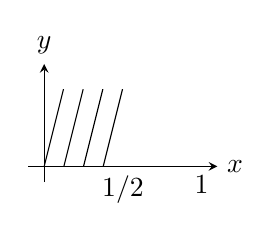
\begin{tikzpicture}[scale=1.0, >=stealth]
  \draw[->] (-0.2,0) -- (2.2,0) node[right] {$x$};
  \draw[->] (0,-0.2) -- (0,1.3) node[above] {$y$};
  \foreach \k in {0,1,2,3}{
    \draw[domain=0:0.98, smooth] plot ({\k/4+\x*0.25},{\x});
  }
  \node[below] at (1,0) {$1/2$};
  \node[below] at (2,0) {$1$};
\end{tikzpicture}
\quad
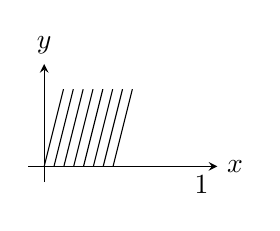
\begin{tikzpicture}[scale=1.0, >=stealth]
  \draw[->] (-0.2,0) -- (2.2,0) node[right] {$x$};
  \draw[->] (0,-0.2) -- (0,1.3) node[above] {$y$};
  \foreach \k in {0,1,2,3,4,5,6,7}{
    \draw[domain=0:0.98, smooth] plot ({\k/8+\x*0.125*2},{\x});
  }
  \node[below] at (2,0) {$1$};
\end{tikzpicture}
\end{center}
（$y=f_2(x)$，$y=f_3(x)$）

又，式にして，$k=0,1,\cdots,7$に対し
\[
f_3(x)=8x-k \quad\left(\frac{k}{8}\le x<\frac{k+1}{8}\right), \qquad f_3(1)=1
\]

\textbf{(2)} (1)以下同様に，$f_n(x)=2^nx-t\ \left(\dfrac{t}{2^n}\le x<\dfrac{t+1}{2^n}\right)$，$f_n(1)=1$（$t=0,1,\cdots,2^n-1$）であること$\cdots\diamondsuit$を帰納的に示す。$n=\ell\ (\ell\in\mathbb{N})$での$\diamondsuit$の成立を仮定すると，①から，
\[
f_{\ell+1}(x)=
\begin{cases}
2(2^\ell x-t) & \left(\dfrac{t}{2^\ell}\le x<\dfrac{t+1/2}{2^\ell}\right) \\
2(2^\ell x-t)-1 & \left(\dfrac{t+1/2}{2^\ell}\le x<\dfrac{t+1}{2^\ell}\right)
\end{cases}
\]
つまり
\[
f_{\ell+1}(x)=
\begin{cases}
2^{\ell+1}x-2t & \left(\dfrac{2t}{2^{\ell+1}}\le x<\dfrac{2t+1}{2^{\ell+1}}\right) \\
2^{\ell+1}x-(2t+1) & \left(\dfrac{2t+1}{2^{\ell+1}}\le x<\dfrac{2t+2}{2^{\ell+1}}\right)
\end{cases}
\]
だから，$f_{\ell+1}(1)=1$とあわせて，$f_{\ell+1}(x)=2^{\ell+1}x-t'\ \left(\dfrac{t'}{2^{\ell+1}}\le x<\dfrac{t'+1}{2^{\ell+1}}\right)$となり，$n=\ell+1$でも$\diamondsuit$は成立。よって任意の$n\in\mathbb{N}$で$\diamondsuit$は成立。

従って，$1\le\ell\le n$なる自然数$\ell$に対し
\[
f_\ell(p)=2^\ell p-t_p \quad(\text{ただし}\ t_p\text{は}\ t_p/2^\ell\le p<(t_p+1)/2^\ell\text{をみたす0以上の整数}) \quad\cdots\text{②}
\]
と書ける。ところで，$n\to\infty$を考えるので$n$は$m$より大きいとして良く，$m\le n$で考えれば良い。$\cdots$③
\[
\frac{t_p}{2^\ell}\le\frac{k}{2^m}<\frac{t_p+1}{2^\ell} \iff k\cdot2^{\ell-m}-1<t_p\le k\cdot2^{\ell-m} \quad\cdots\text{③}
\]
である。$\ell\ge m$の時，③の両辺は整数（1つ差）で$t_p\in\mathbb{Z}$だから右側の等号が成立し，この時$f_\ell(p)=0$である。したがって，$\ell=1,2,\cdots,m$で和をとれば良い（$\because$③）。
\[
\sum_{\ell=1}^nf_\ell(p)=\sum_{\ell=1}^mf_\ell(p)=A \quad(n\text{に関係ない定数})
\]
だから，
\[
(\text{与式})=\frac{A}{n}\xrightarrow{n\to\infty}0
\]
となる。
\end{proof}

\newpage

\section*{第5問}

\begin{proof}[解]
\[
I_n=(-1)^n\int_0^{\frac{\pi}{4}}\frac{x\cos(2n-1)x}{\cos x}dx
\]
である。

\textbf{(1)}
\[
I_n-I_{n-1}=(-1)^n\left[\int_0^{\frac{\pi}{4}}\frac{x\cos(2n-1)x}{\cos x}dx+\int_0^{\frac{\pi}{4}}\frac{x\cos(2n-3)x}{\cos x}dx\right]
\]
\[
=(-1)^n\int_0^{\frac{\pi}{4}}\frac{x\{\cos(2n-3)x+\cos(2n-1)x\}}{\cos x}dx
\]
\[
=(-1)^n\int_0^{\frac{\pi}{4}}\frac{x}{\cos x}\cdot2\cos(2n-2)x\cos x\,dx
\]
\[
=(-1)^n\int_0^{\frac{\pi}{4}}2x\cos(2n-2)x\,dx \quad\cdots\text{①}
\]
これは$n\ge2$であることから
\[
\int_0^{\frac{\pi}{4}}2x\cos(2n-2)x\,dx=2\left[\frac{x}{2n-2}\sin(2n-2)x+\frac{1}{(2n-2)^2}\cos(2n-2)x\right]_0^{\frac{\pi}{4}}
\]
\[
=2\left\{\frac{\pi}{4}\cdot\frac{1}{2n-2}\sin\frac{n-1}{2}\pi+\frac{1}{(2n-2)^2}\left(\cos\frac{n-1}{2}\pi-1\right)\right\}
\]
だから，①に代入して
\[
I_n-I_{n-1}=2(-1)^n\left\{\frac{\pi}{4}\cdot\frac{1}{2n-2}\sin\frac{n-1}{2}\pi+\frac{1}{(2n-2)^2}\left(\cos\frac{n-1}{2}\pi-1\right)\right\}
\]

\textbf{(2)} $I_1=-\displaystyle\int_0^{\frac{\pi}{4}}x\,dx=-\frac12\left(\frac{\pi}{4}\right)^2$だから，(1)で$n=2,3$として
\[
I_2=I_1+2\left(\frac{\pi}{4}\cdot\frac12-\frac14\right)=I_1+\frac{\pi}{4}-\frac12
\]
\[
I_3=I_2-2\left(\frac{\pi}{4}\cdot\frac14\cdot0-\frac18\right)=I_2+\frac14
\]
\[
\therefore\ I_3=I_1+\frac{\pi}{4}-\frac12+\frac14=-\frac{\pi^2}{32}+\frac{\pi}{4}-\frac14
\]
である。
\end{proof}

\end{document}
